%!TEX encoding = UTF-8 Unicode
%!TEX root = ../compendium2.tex

\Lab{\LabWeekEIGHT}

\begin{Goals}
\item Kunna skapa och använda matriser.
\item Kunna iterera över matriser med nästlade for-loopar.
\item Träna på algoritmkonstruktion.
\item Använda en integrerad utvecklingsmiljö (IDE).
\end{Goals}

\begin{Preparations}
\item Gör övning {\tt \ExeWeekEIGHT} i kapitel \ref{chapter:W08}, speciellt övning \ref{exe:matrices:labprep}.

\item Läs igenom hela laborationen och studera den befintliga koden i \TODO \code{workspace}.

\item Läs appendix \ref{appendix:ide} och välj vilken IDE du ska använda (ScalaIDE/Eclipse eller IntelliJ IDEA). Säkerställ att du får igång en av dessa utvecklingsmijöer genom att köra hello-world-exemplet och sedan ladda ner och importera kursens \TODO workspace enligt instruktionerna i appendix \ref{appendix:ide}.
\end{Preparations}


\begin{figure}[H]
  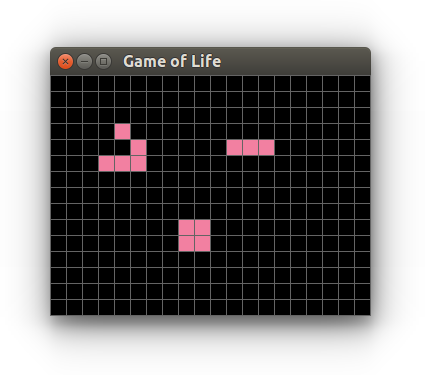
\includegraphics[width=0.8\textwidth]{../img/glider-blinker-block}

  \vspace{-2em}\label{lab:life:glider-blinker-block}\caption{Ett universum med 15 rader och 20 kolumner. Cellkolonin innehåller tre cellgrupper: ett s.k. rymdskepp av typen \emph{glider}, en \emph{blinker} och ett \emph{block}.}
\end{figure}



\subsection{Bakgrund}


\emph{Game of Life} simulerar en koloni av encelliga organismer som lever, förökar sig och dör i en matris, enligt några enkla men väl valda regler som konstruerades av matematikern John Horton Conway på 1970-talet. Spelet går ut på att simulera flera generationer utifrån en startkonfiguration, även kallad \emph{cellkoloni}, där varje enskild cells överlevnad beror på dess omgivning. Spelet har inga medvetna spelare och om reglerna följs så kommer slutresultatet enbart bero på startkonfigurationen.



I \emph{Game of Life} består universum av en matris med celler som är antingen levande eller döda. Varje cell har 8 stycken \emph{grannar}, som utgörs av de närmsta omgivande cellerna vertikalt, horisontellt och diagonalt. Varje cells tillstånd i nästa generation bestäms av följande regler:
\begin{enumerate}[nolistsep]
    \item \textbf{Fortlevnad}. Om en levande cell har två eller tre grannar så lever den vidare.
    \item \textbf{Död}. Om en levande cell har mindre än två eller mer än tre grannar så dör den av underpopulation respektive överpopulation.
    \item \textbf{Födelse}. Om cellen är död och har exakt tre grannar så föds den och dess tillstånd ändras till levande, annars fortsätter den vara död.
\end{enumerate}

Flera cellkolonier uppvisar ett ''levande'' beteende där cellmatrisen koloniseras på intressanta vis när en sekvens av generationer visualiseras. Detta är ett exempel på \emph{emergent} beteende där komplexa, självorganiserade strukturer kan uppstå ur tillsynes enkla förutsättningar.

Läs mer om \emph{Game of Life} på Wikipedia:
\begin{itemize}[noitemsep,topsep=0pt]
    	\item \url{https://en.wikipedia.org/wiki/Conway's_Game_of_Life}
    	\item \url{https://sv.wikipedia.org/wiki/Game_of_Life}
\end{itemize}

\subsection{Obligatoriska krav}

Följande funktionella krav ska uppfyllas av ditt program:
\begin{itemize}[nosep, label={$\square$},]
\item Levande celler ska ha den rosa\footnote{\url{https://www.dsek.se/aktiva/grafiskprofil/farg.php}} RGB-färgen \code{(242, 128, 161)}.
\item Döda celler ska vara svarta.
\item Universum ska ritas som ett rutnät med smala, grå linjer.
\item Tangenttryckningar och musklick ska fungera enligt följande hjälptext, som ska skrivas ut då programmet startas:
\begin{Code}
  val help = """
    Welcome to GAME OF LIFE!

    Click on cell to toggle.
    Press ENTER for next generation.
    Press SPACE to toggle play/stop.
    Press R to create random life.
    Press BACKSPACE to clear life.
    Close window to exit.
  """
\end{Code}
Då \emph{play} aktiveras med blankstegstangenten ska en kontinuerlig simulering av universum fortgå där varje ny generation visualiseras med en lagom fördröjning emellan generationer, tills simuleringen stoppas, t.ex. genom tryck ånyo på blankstegstangenten. Med \emph{Enter}-tangenten visas \emph{en} efterkommande generation och ev. pågående simulering stoppas. Vid musklick på en cell växlas dess livstillstånd från levande till död eller vice versa. Ett tryck på backstegstangenten renderar alla cellers i universum död. Ett tryck på R ska ge slumpmässigt liv med lika sannolikhet för död respektive levande cell i varje position.

\end{itemize}

\vspace{1em}\noindent Din kod ska utformas enligt dessa design-krav:
\begin{itemize}[nosep, label={$\square$}]
\item
\end{itemize}



\subsection{Valbara krav -- välj minst ett}

Du ska implementera minst ett (gärna flera) av dessa krav:
\begin{itemize}[nosep, label={$\square$}]
\item
\end{itemize}



\subsection{Tips och förslag}

\begin{enumerate}[leftmargin=*]
\item \textbf{Använda IDE.}
\end{enumerate}

\noindent\TODO Är det något mer tips som behövs för att labben ska gå smidigt?
